\section{Analysis and Discussion}

\subsection{Chain-of-Thought Helps Through Different Mechanisms}

\begin{figure*}[t]
\centering
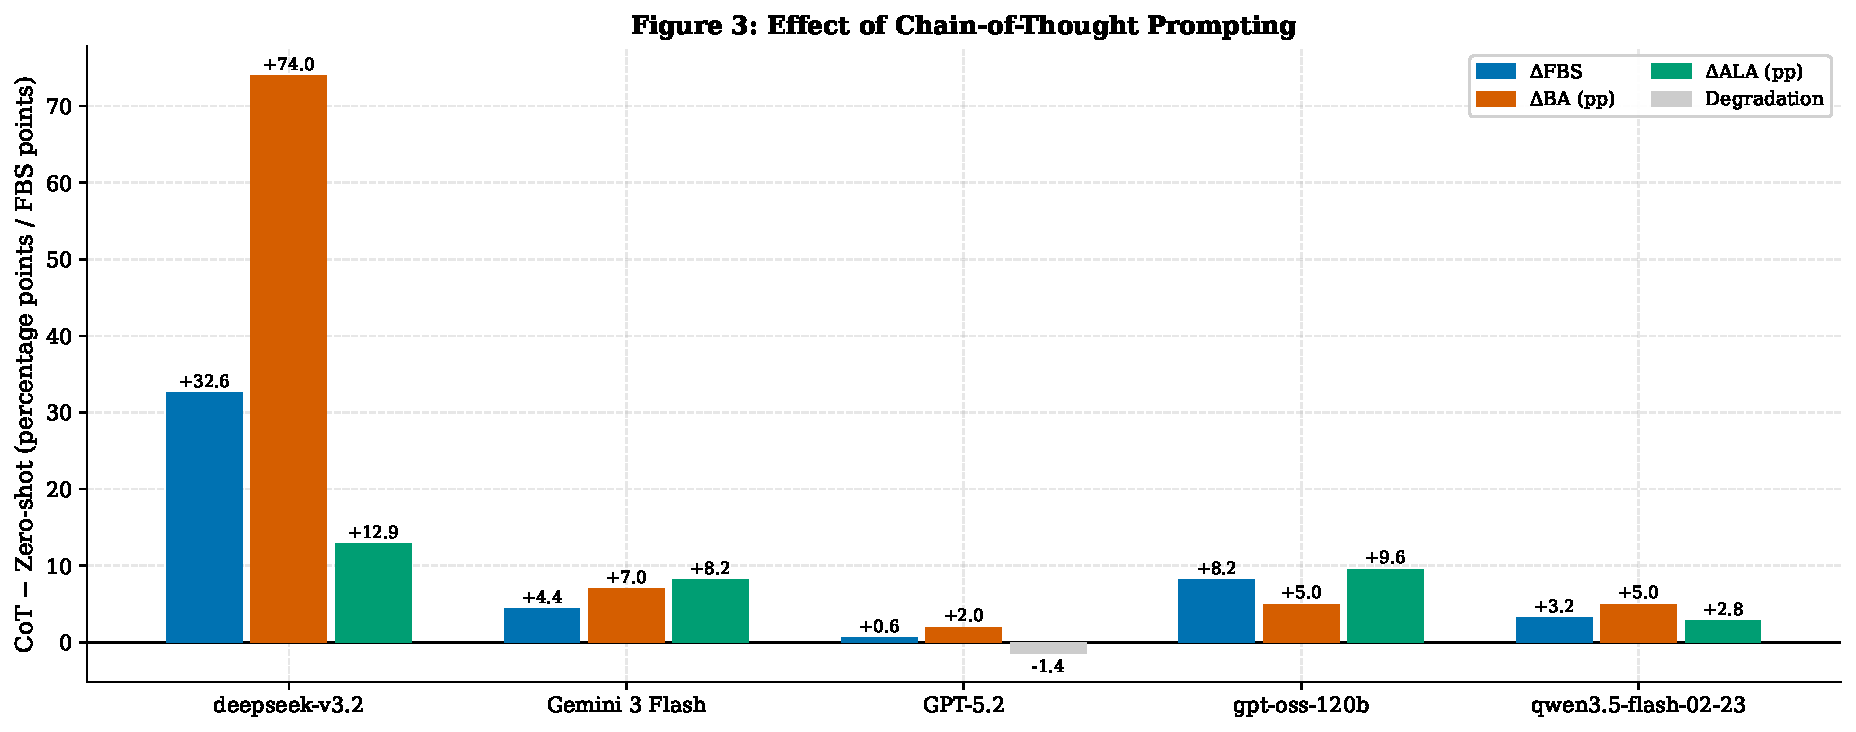
\includegraphics[width=0.95\textwidth]{../figures/F3_cot_effect.pdf}
\caption{Effect of chain-of-thought prompting on the completed
500-problem study.}
\label{fig:cot-effect}
\end{figure*}

Figure~\ref{fig:cot-effect} shows that \CoT{} delivers heterogeneous
gains across model families.
GPT-5.4 Nano benefits the most (\(+55.52\) \fbs{} points, \(495\) of
\(500\) problems improve), followed by Grok~4.1 Fast (\(+45.33\),
\(491\) improve), DeepSeek-v3.2 (\(+41.43\), \(469\) improve), and
Qwen~3.5 Flash (\(+36.40\), \(477\) improve).
Gemini~3 Flash shows a smaller gain (\(+8.63\)).
For GPT-5.4 Nano, the gain is dramatic: mean arithmetic errors drop by
\(5.13\) per problem, and \CoT{} also recovers \(31\) parse failures
that occur under zero-shot prompting.
DeepSeek-v3.2's gain is primarily arithmetic:
mean arithmetic errors drop by \(3.78\) per problem, and closing-entry
compliance rises by \(27\) percentage points.
Gemini~3 Flash is different: \(275\) problems improve but \(190\)
decline, so its average benefit concentrates on harder problems.

\subsection{Retained Earnings Is the Hardest Account}

\begin{table}[t]
\centering
\small
\resizebox{\columnwidth}{!}{%
\begin{tabular}{lrrrrr}
\toprule
Account & $n$ & Omit & Arith. & Correct & Score \\
 &  & (\%) & (\%) & (\%) &  \\
\midrule
Retained Earnings & 5947 & 76.9 & 17.8 & 5.3 & 0.532 \\
Owner's Equity & 6005 & 0.3 & 70.3 & 29.5 & 0.283 \\
Cash & 6005 & 0.1 & 48.6 & 51.3 & 0.195 \\
Allowance for Doubtful Accts. & 1276 & 18.1 & 14.1 & 67.8 & 0.165 \\
Accounts Receivable & 4438 & 1.2 & 32.8 & 66.0 & 0.139 \\
Accum.\ Depreciation & 2409 & 20.9 & 1.2 & 77.9 & 0.130 \\
Inventory & 5016 & 0.0 & 29.0 & 71.0 & 0.116 \\
Accounts Payable & 4227 & 0.1 & 22.4 & 77.4 & 0.091 \\
\bottomrule
\end{tabular}
}
\caption{Hardest accounts in the Large-500 account-difficulty index,
aggregated over completed model--prompt combinations.}
\label{tab:account-difficulty}
\end{table}


Table~\ref{tab:account-difficulty} aggregates account-level behavior
over the completed Large-500 runs.
The account difficulty index combines omission and arithmetic error
patterns to identify which accounts are hardest to predict reliably.
Retained Earnings is by far the hardest account, with a \(76.9\%\)
omission rate, a \(17.8\%\) arithmetic-error rate, and only a
\(5.3\%\) correct prediction rate.
The next hardest account, Owner's Equity, reveals a different failure
mode: it is almost never omitted, but it is numerically wrong on
\(70.3\%\) of its occurrences.
The benchmark is therefore exposing not just missing terminology but
systematic confusion about how income-statement activity closes into
equity.

\begin{figure*}[t]
\centering
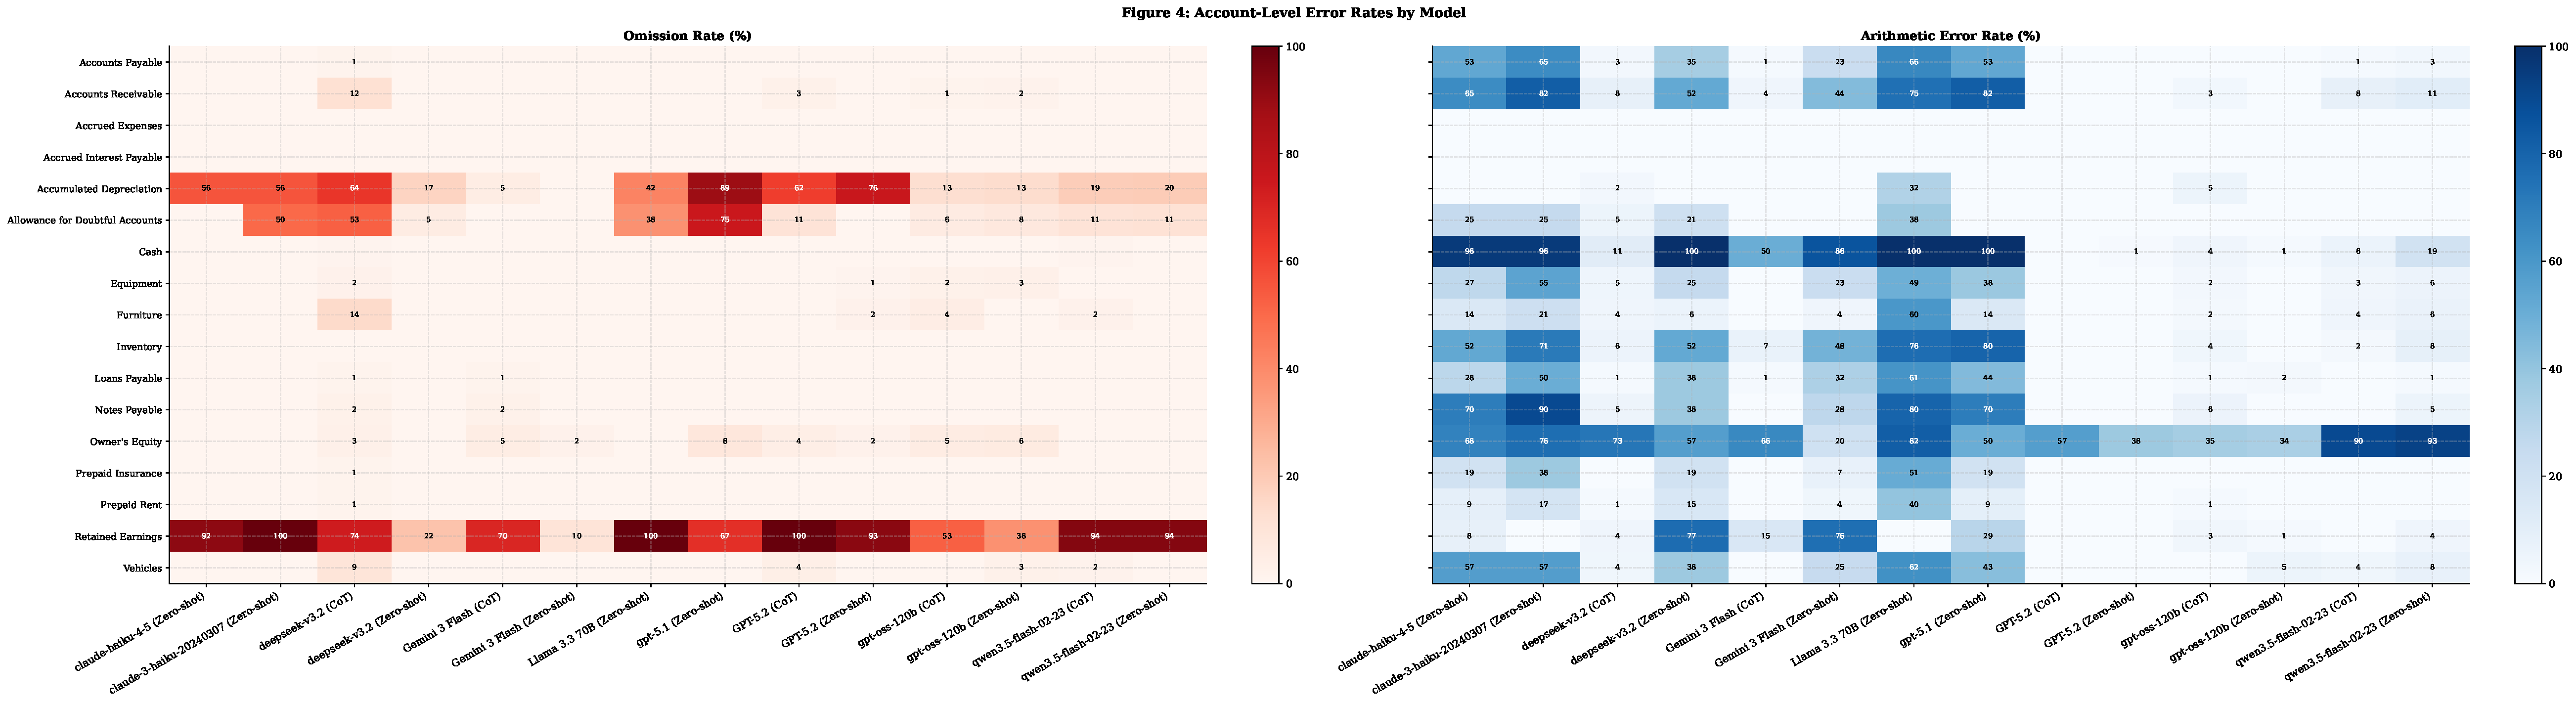
\includegraphics[width=0.95\textwidth]{../figures/F4_account_heatmap.pdf}
\caption{Account omission and arithmetic patterns by model--prompt pair
on the completed 500-problem study.}
\label{fig:account-heatmap}
\end{figure*}

Figure~\ref{fig:account-heatmap} makes this pattern more explicit.
Several otherwise strong \CoT{} runs still omit the closing-entry
transfer:
Grok~4.1 Fast \CoT{} omits Retained Earnings on \(99.6\%\) of the
problems where it is expected, GPT-5.4 Nano \CoT{} on \(99.2\%\),
Gemini~3 Flash \CoT{} and Qwen~3.5 Flash \CoT{} on \(94.3\%\), and
Qwen~3.6 Plus \CoT{} on \(91.3\%\).
The zero-shot runs show the opposite pattern.
They usually include the account, but miscompute it badly, with
Retained Earnings arithmetic-error rates reaching \(80.8\%\)
(DeepSeek-v3.2~\zs{}), \(77.6\%\) (Gemini~3 Flash~\zs{}), and
\(14.6\%\) (Nemotron~3 Super~\zs{}, which instead omits the account on
\(85.4\%\) of problems).
These results identify at least two closing-entry failure modes:
omission and numeric corruption.

\subsection{Factor Sensitivity Still Separates Robust Models from Fragile Ones}

A detailed factor-sensitivity summary appears in
Appendix Table~\ref{tab:complexity-factors}.
It reports each model--prompt pair's
most harmful \emph{controlled} factor, together with the coefficient of
variation of its difficulty curve.
No single mechanism hurts every model in the same way, so robustness
and factor sensitivity must be read together.
DeepSeek-v3.2 \CoT{} and Qwen~3.6 Plus \CoT{} are nearly invariant even
to their worst factor, with controlled drops of only \(1.2\) and
\(1.7\) \fbs{} points.
Qwen~3.5 Flash \CoT{}, by contrast, loses \(10.8\) points on
mixed-funding problems after controlling for difficulty.
Only three \CoT{} runs achieve a difficulty-curve CV below \(3\%\):
Grok~4.1 Fast, DeepSeek-v3.2, and GPT-5.4 Nano.
DeepSeek-v3.2 is the only model with a reverse difficulty curve, while
all zero-shot runs except Gemini~3 Flash exhibit cliff behavior.
